
\begin{figure}
\centering
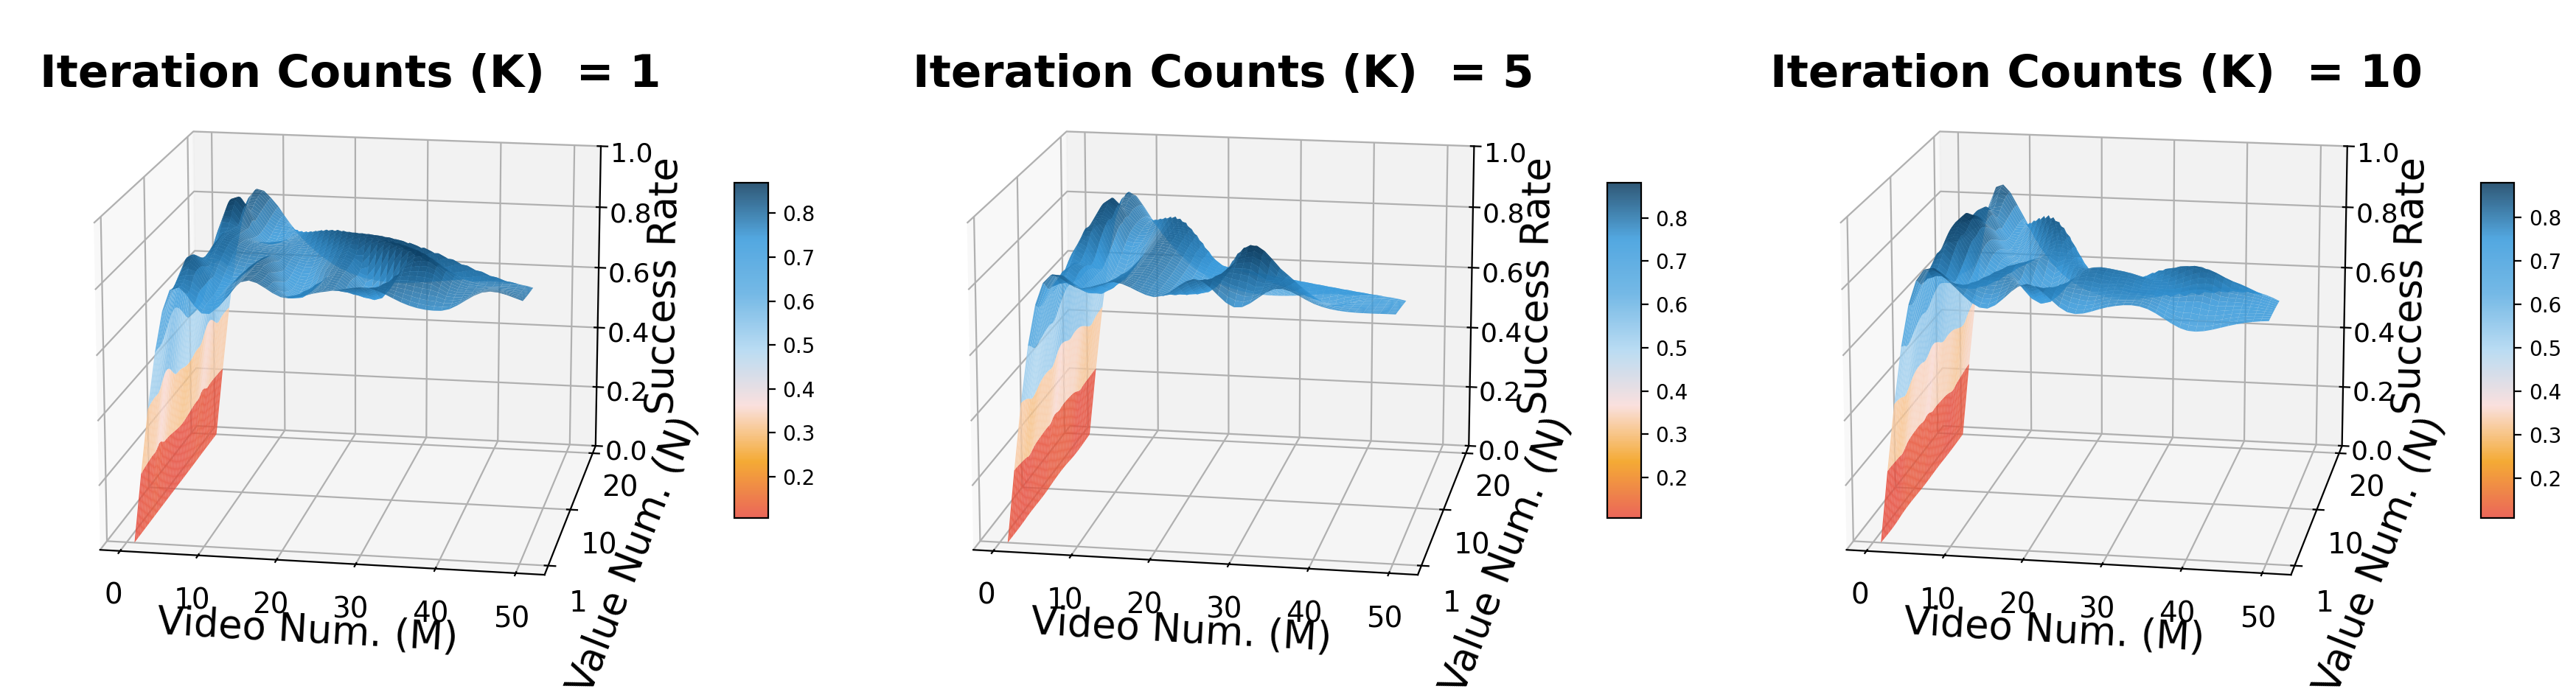
\includegraphics[width=0.8\textwidth]{figures/stage1_main.png}
\caption{
WAV performance under varying iteration counts $K$, video latent noise sampling numbers $M$, and trajectory value noise sampling numbers $N$.
}
  \label{fig:stage1_main}
\end{figure}

\paragraph{Effect of Iteration Counts $K$ and Sampling Sizes $M, N$.}
As shown in Fig.~\ref{fig:stage1_main}, 

increasing $K$ from 1 to 5 leads to a clear improvement in success rate, indicating that iterative latent planning effectively refines the trajectory distribution toward high-value regions. 
However, further increasing $K$ to 10 yields only marginal gains, suggesting diminishing returns from excessive iterations. 
In contrast, the performance is highly sensitive to $M$, where increasing the number of video samples results in a steep improvement, especially in the low-sample regime. 
This highlights the importance of sufficiently exploring future trajectory hypotheses. 
The influence of $N$ is comparatively milder, with performance saturating earlier, indicating that dense value evaluation provides limited additional benefit once a reasonable estimation is achieved.
More results are given in Appendix Fig.~\ref{app_fig:stage1}.
Appendix Fig.~\ref{app_fig:value} and~\ref{app_fig:gt_pred_libero} compare trajectory value and video predictions to ground truth, respectively.

\begin{wrapfigure}{r}{0.53\textwidth}
\centering
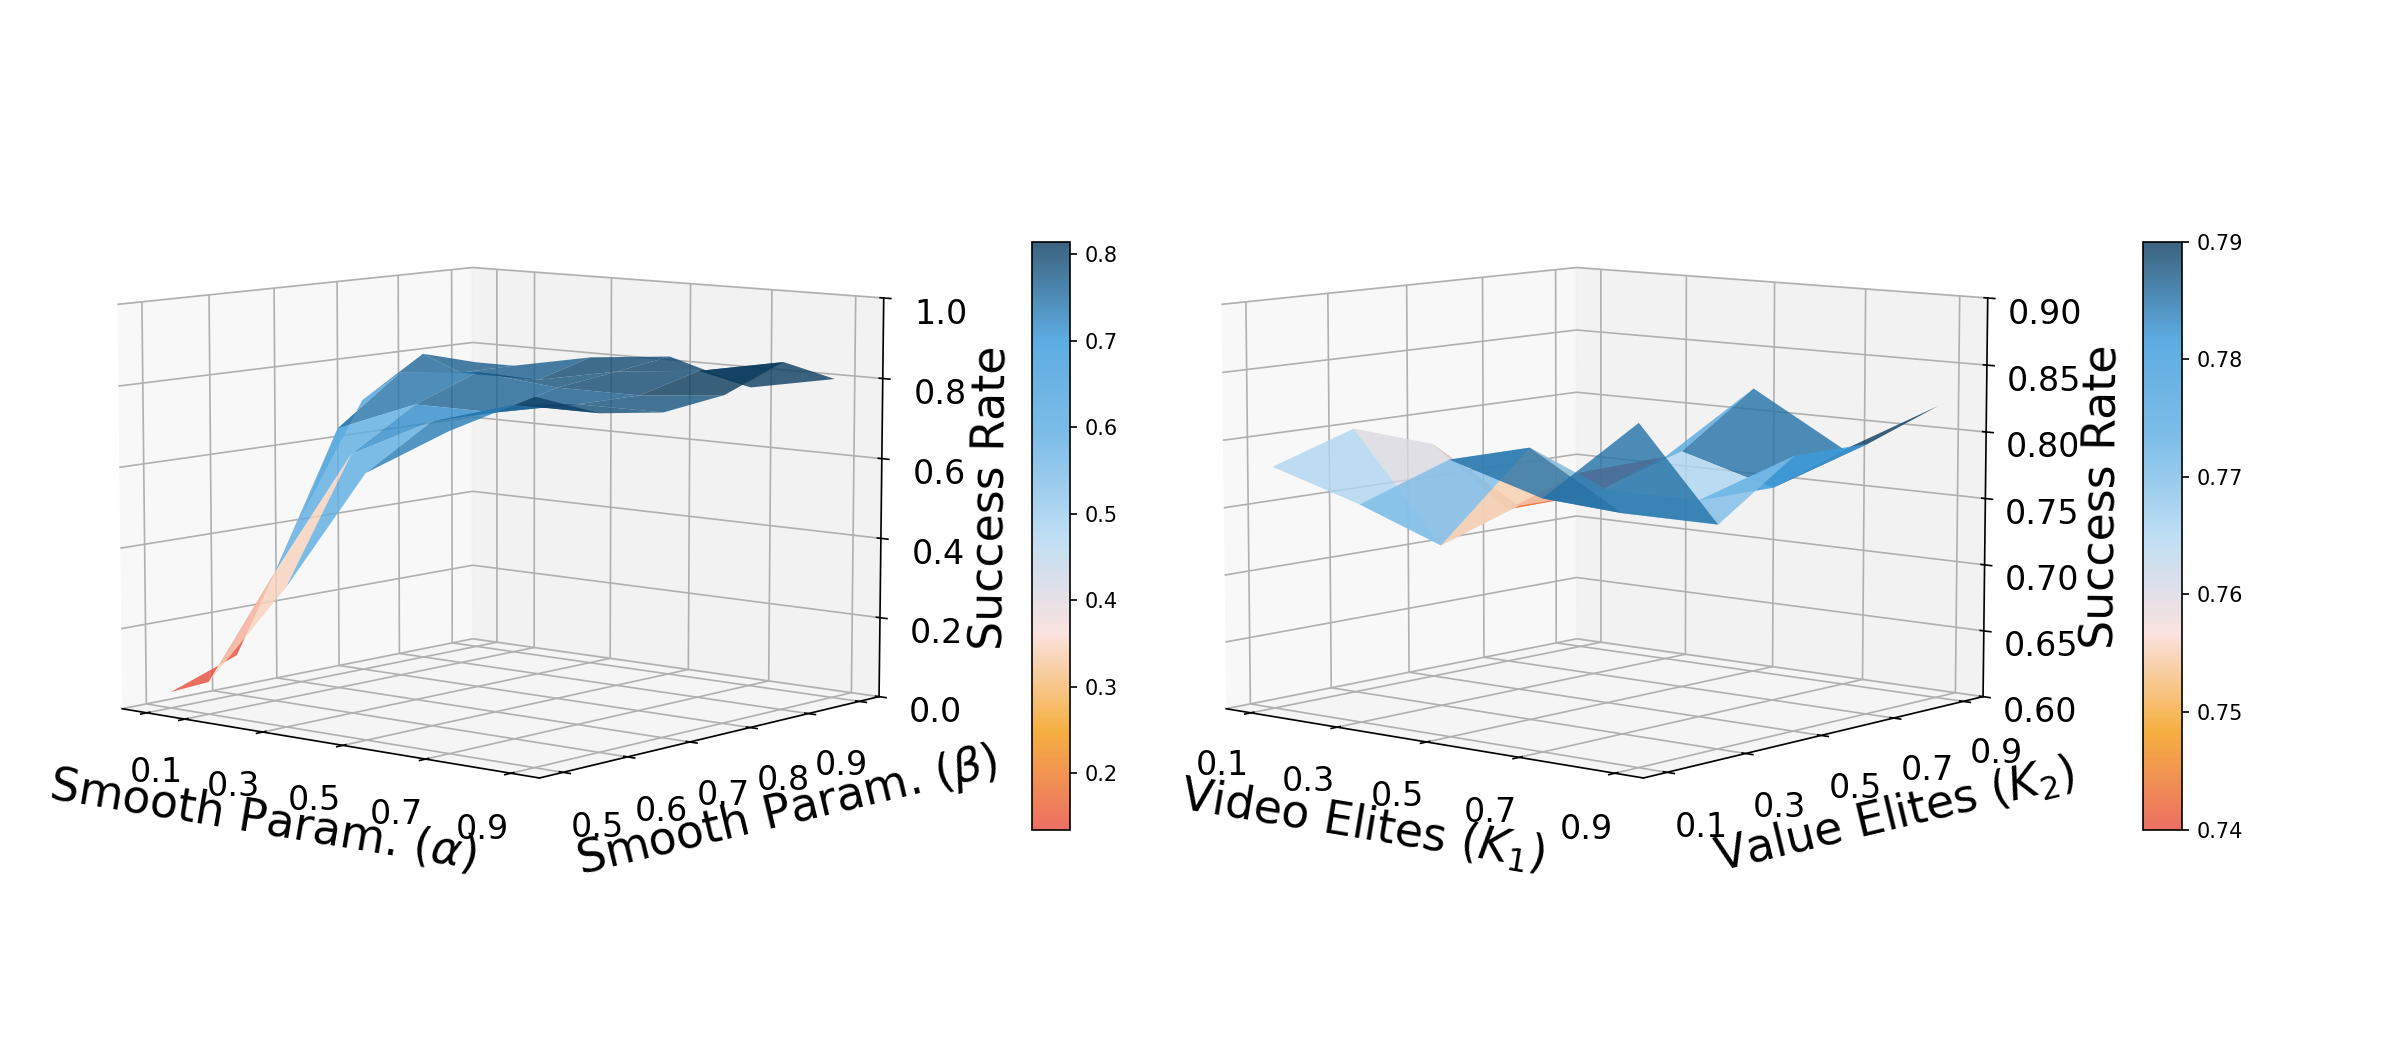
\includegraphics[width=0.95\linewidth]{figures/stage2_stage3_vis.png}
\caption{

\textbf{Left:} WAV sensitivity to smoothing parameters $\alpha$ and $\beta$.
\textbf{Right:} WAV sensitivity to elite counts $K_1$ and $K_2$.
}
  \label{fig:stage2_stage3_vis}
\end{wrapfigure}
\paragraph{Effect of Smoothing Parameters ($\alpha, \beta$).}

Fig.~\ref{fig:stage2_stage3_vis} (\textbf{Left}) shows that when $\alpha$ is small, the success rate drops sharply, indicating that insufficient smoothing leads to unstable distribution updates and poor convergence. 
As $\alpha$ increases, performance improves rapidly and then plateaus, showing a clear steep region followed by saturation. A similar but slightly milder trend is observed for $\beta$. This suggests that stabilizing the update of the latent distribution is crucial, but overly strong smoothing provides limited additional benefit once convergence is achieved.

\paragraph{Effect of Elite Selection ($K_1, K_2$).}

Fig.~\ref{fig:stage2_stage3_vis} (\textbf{Right}) shows that the performance is relatively stable across different choices of $K_1$ and $K_2$, indicating that the WAV is not highly sensitive to these parameters. 
However, extremely small values lead to noticeable performance degradation, suggesting that a sufficient number of elite samples is necessary for stable distribution updates.

\begin{wrapfigure}{r}{0.53\textwidth}
\centering
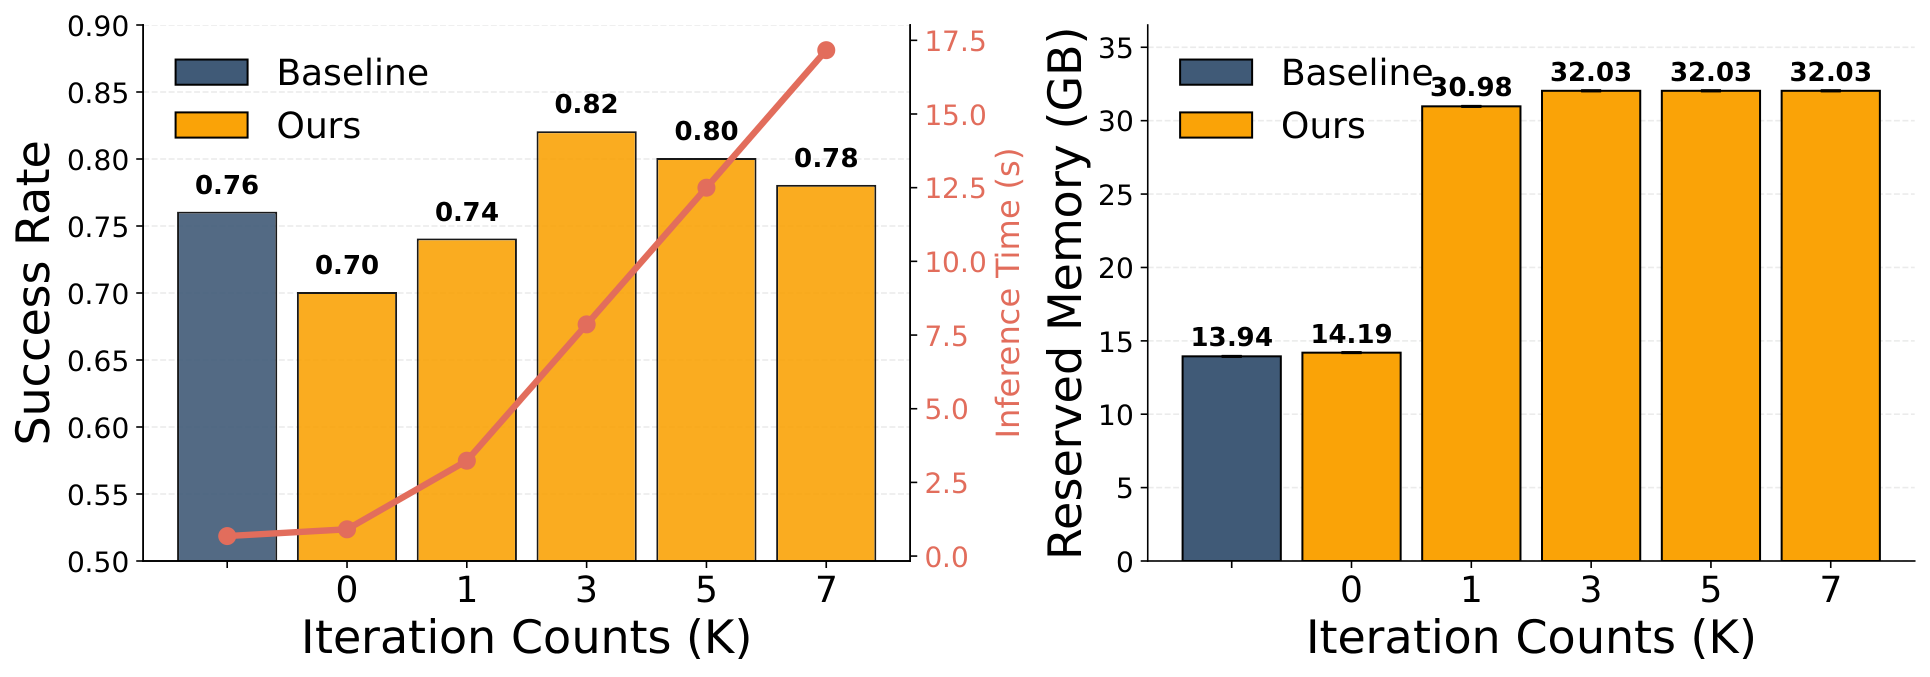
\includegraphics[width=0.95\linewidth]{figures/speed_memory.pdf}
\caption{
Performance and efficiency trade-off of WAV across $K$: success rate and inference time (\textbf{Left}), and GPU memory usage (\textbf{Right}).
Baseline: GE-ACT.
Ours: WAV.
}
\label{fig:speed_acc}
\end{wrapfigure}
\paragraph{Performance--Efficiency Trade-off.} 
Fig.~\ref{fig:speed_acc} shows that increasing the number of iterations from $0$ to $3$ consistently improves performance. 
Beyond $3$ gains saturate while computational cost, particularly inference time, continues to grow. 

Therefore, $K=3$ provides a favorable balance between effectiveness and efficiency, achieving strong performance with moderate computational overhead.
This behavior reflects the diminishing returns of iterative refinement, indicating that a small number of inference steps is sufficient to capture most of the planning benefits.

